\section{Validation of kinematic simulation}
    \subsection{Theoretical evaluation of kinematic parameters}
        In this section, the displacement, velocity and acceleration of the output component is evaluated manually at four positions of the input link separated by 90 degrees. 

        \begin{figure}[hbt!]
            \centering
            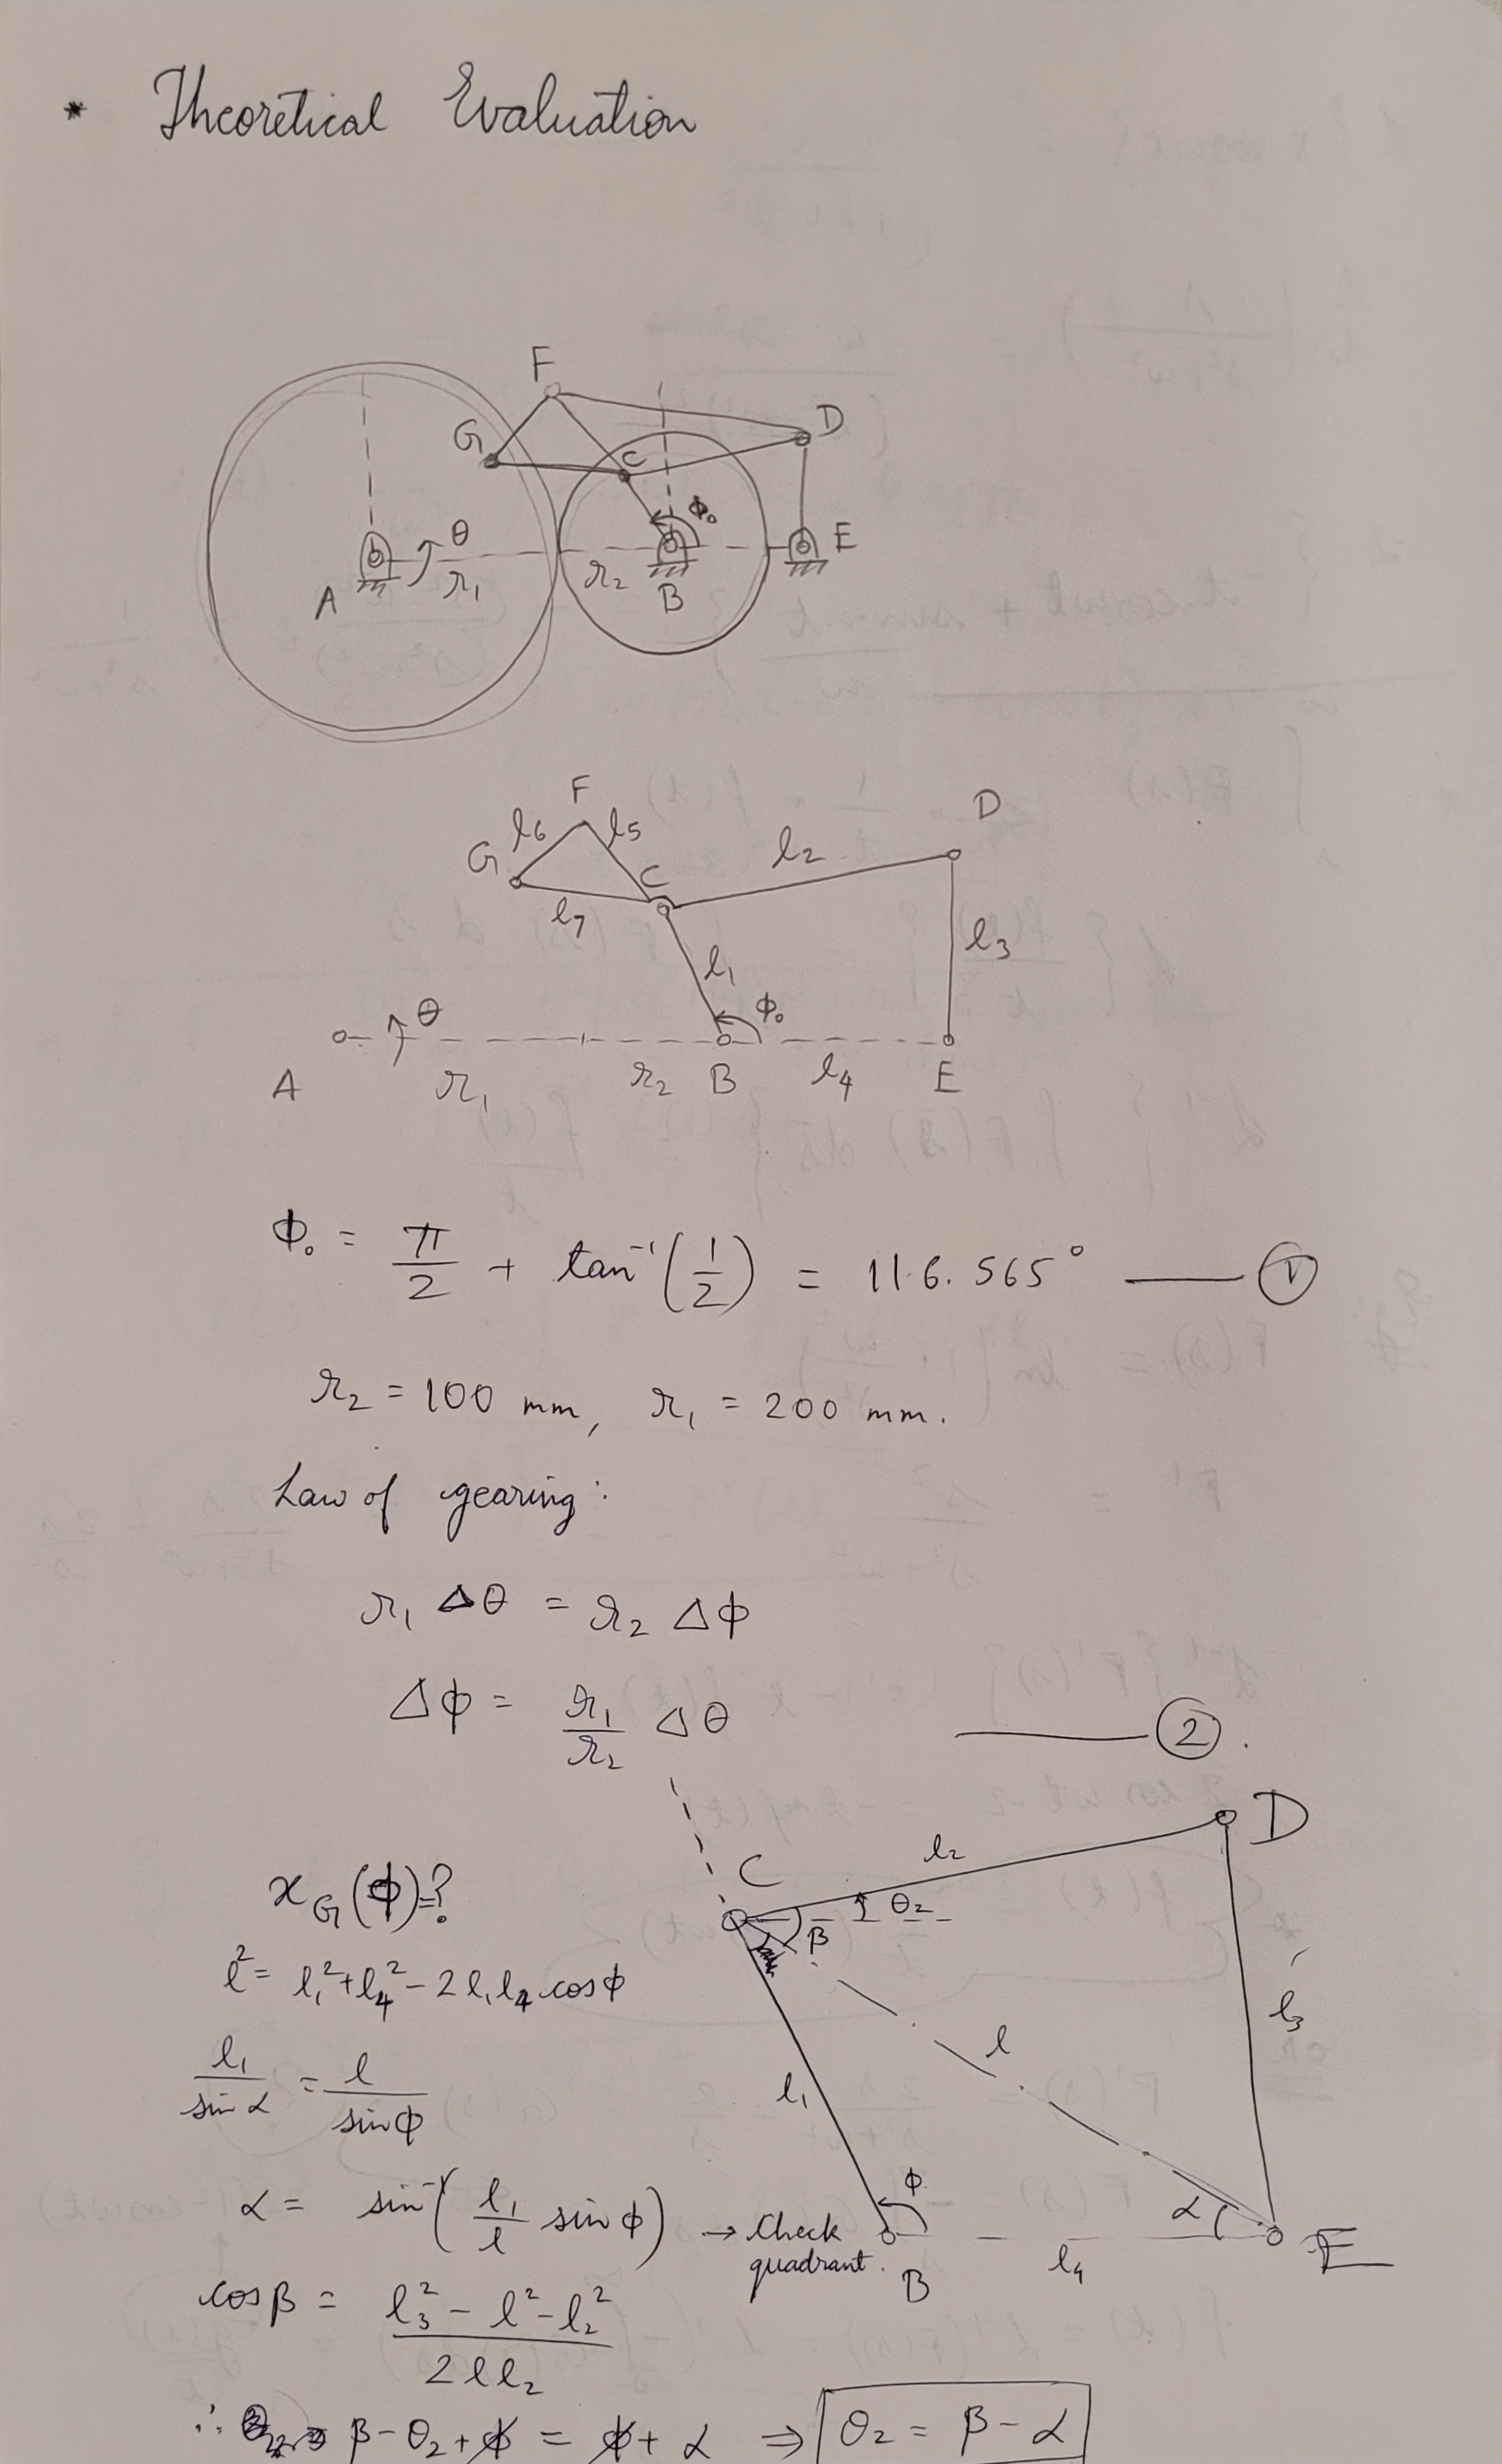
\includegraphics[width=0.9\columnwidth]{Images/Theo_eval1.jpg}
            \caption{Theoretical evaluation page 1}
            \label{fig:theo_eval1}
        \end{figure}

        \begin{figure}[hbt!]
            \centering
            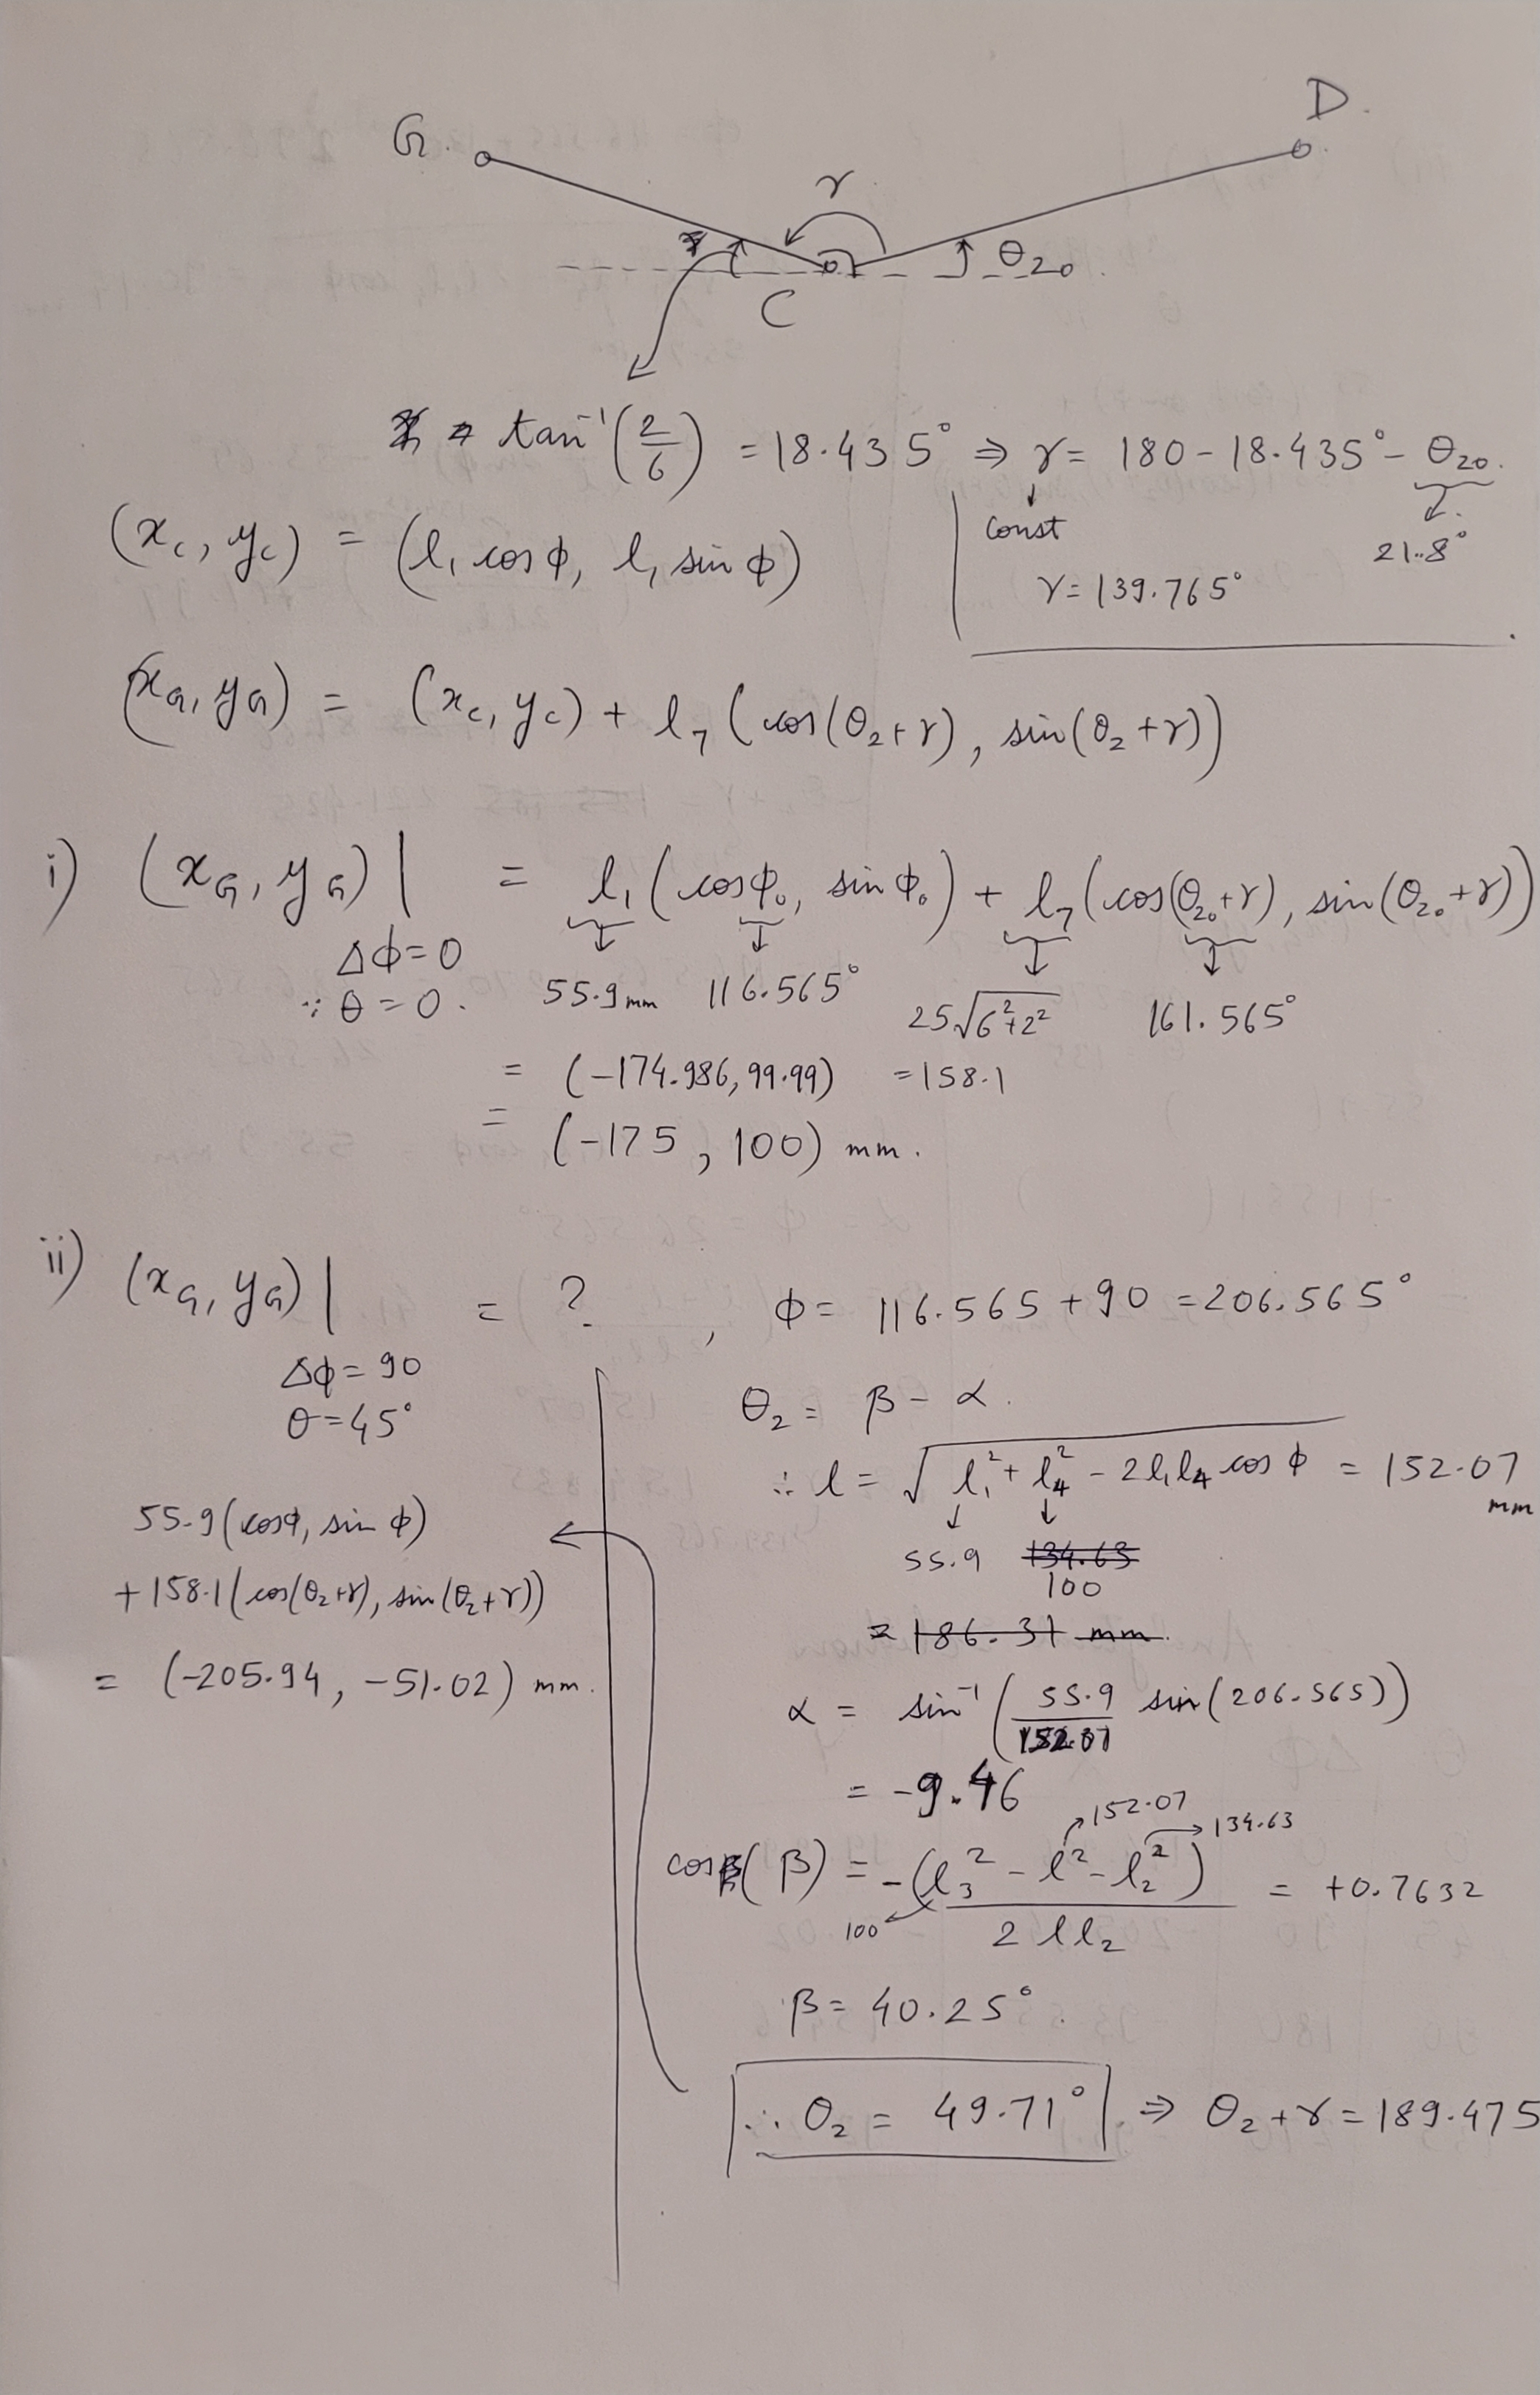
\includegraphics[width=0.9\columnwidth]{Images/Theo_eval2.jpg}
            \caption{Theoretical evaluation page 2}
            \label{fig:theo_eval2}
        \end{figure}

        \begin{figure}[hbt!]
            \centering
            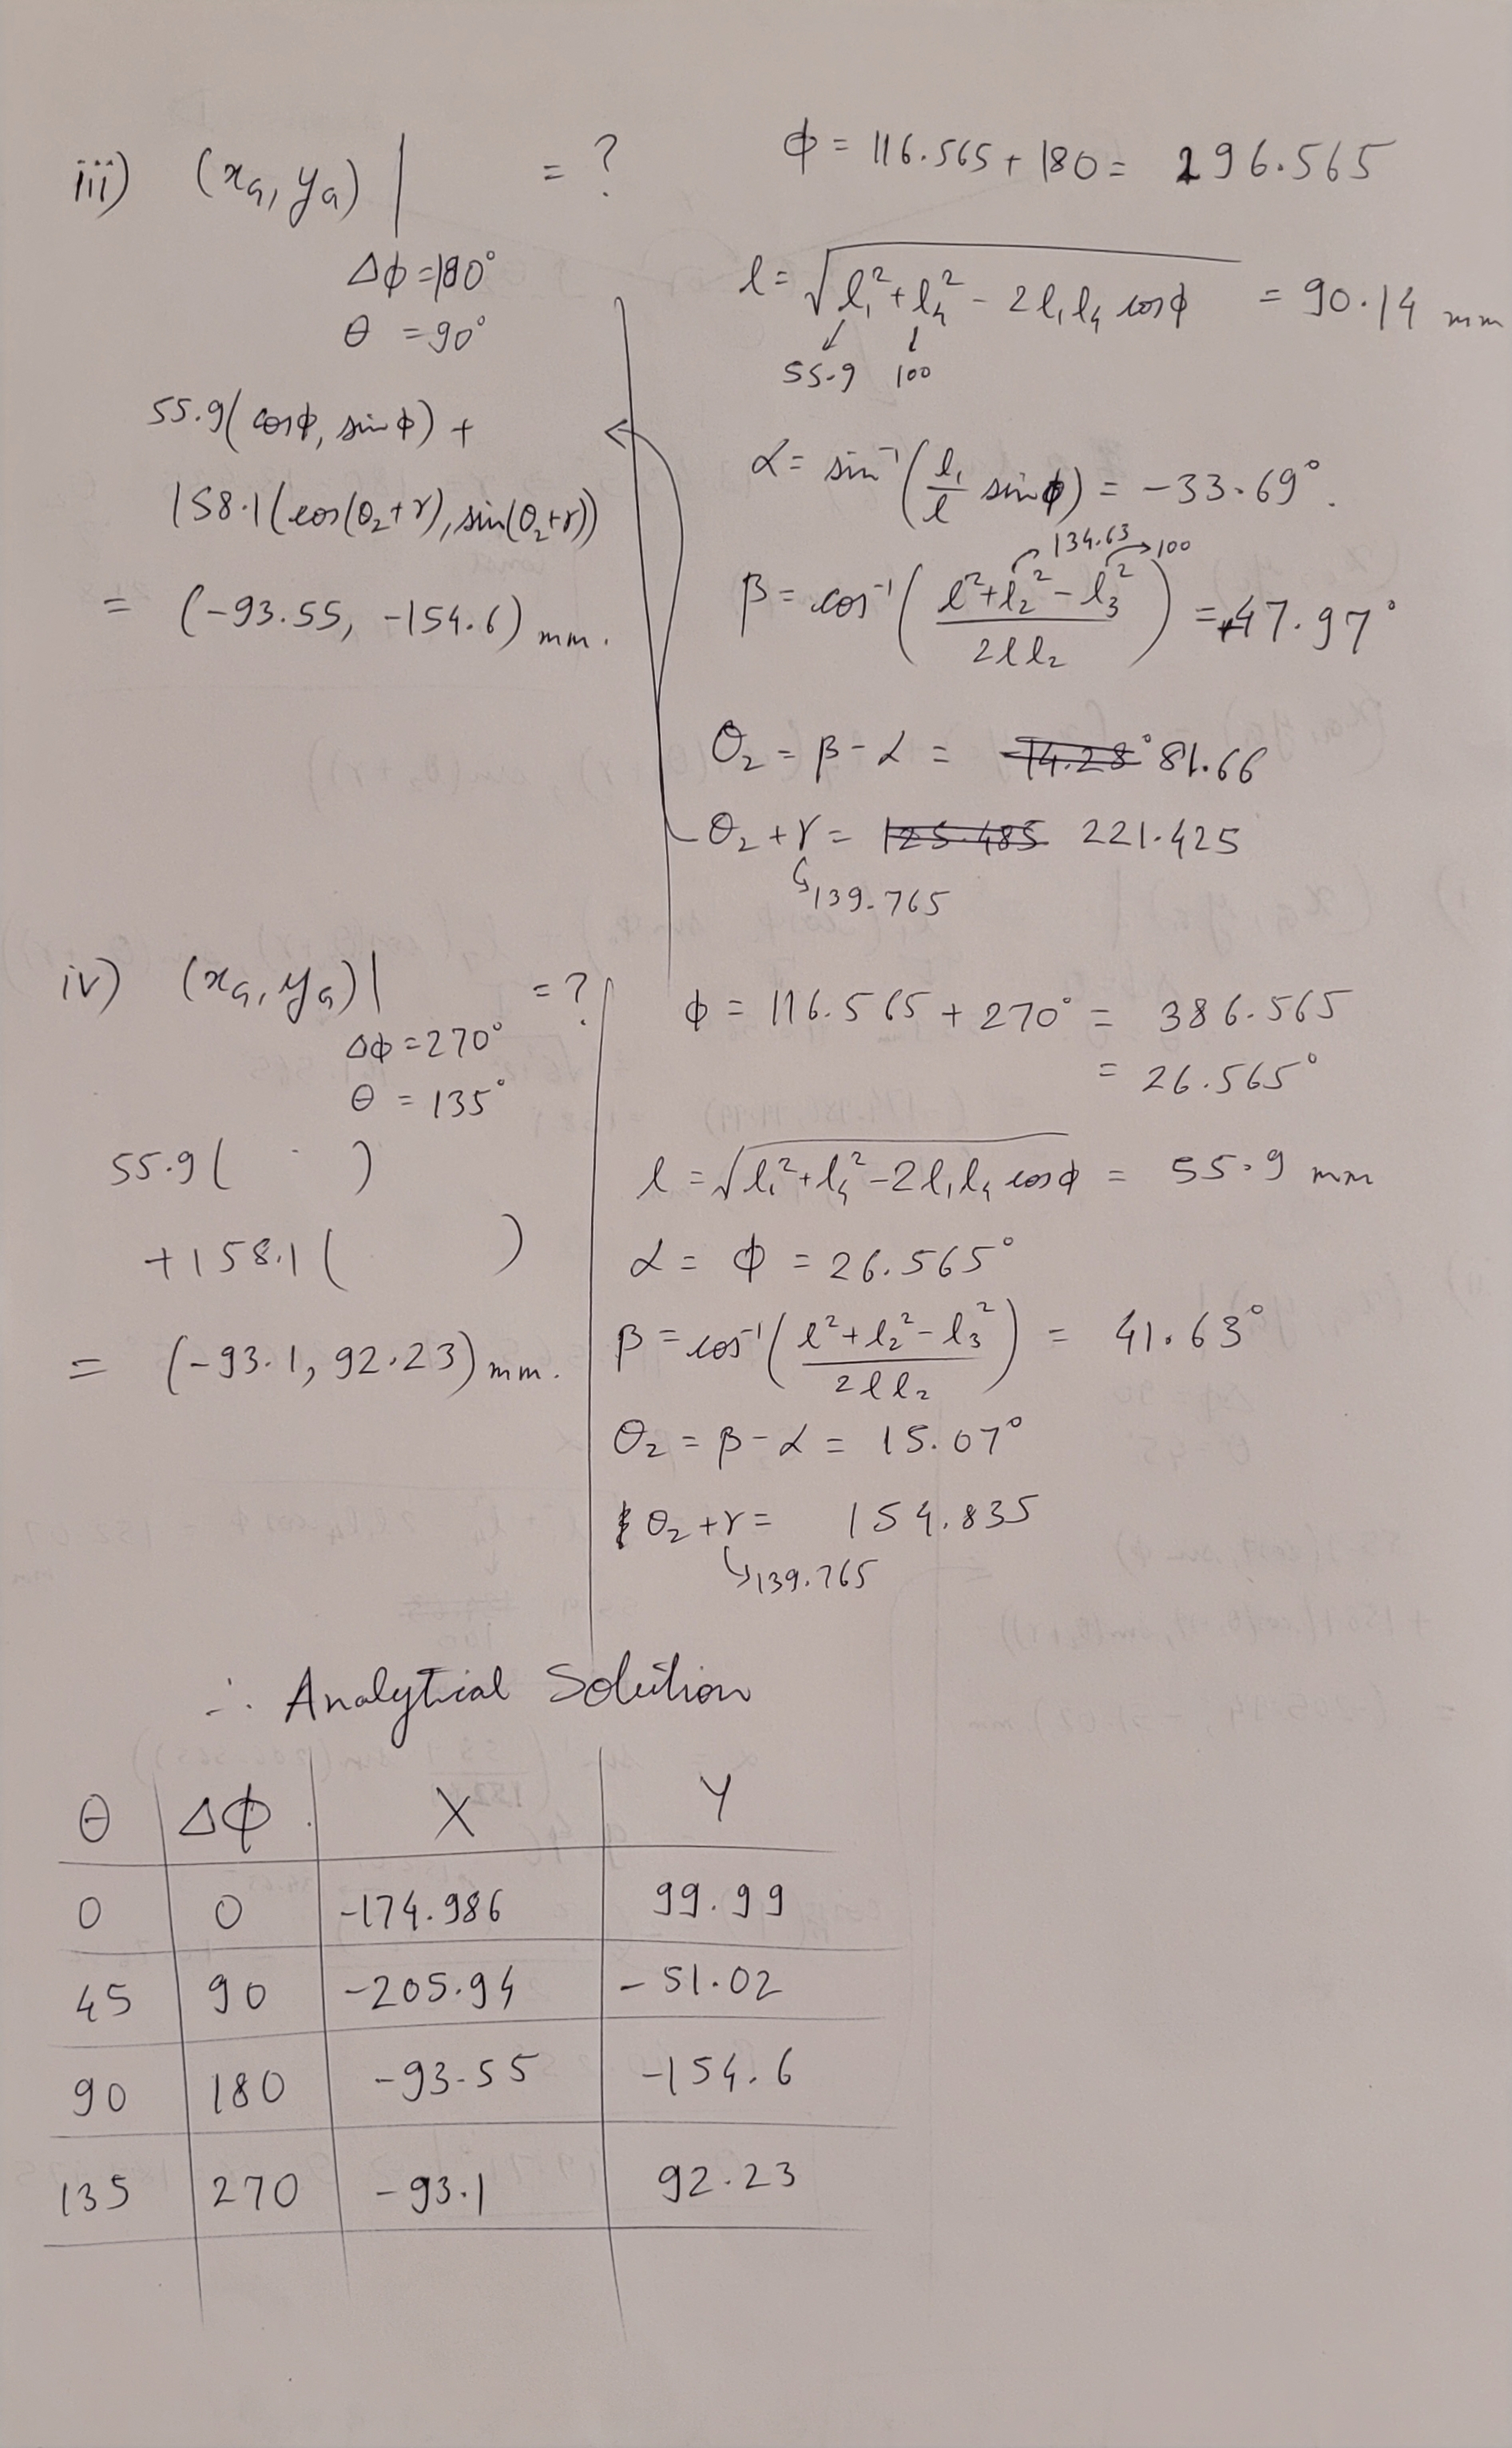
\includegraphics[width=0.9\columnwidth]{Images/Theo_eval3.jpg}
            \caption{Theoretical evaluation page 3}
            \label{fig:theo_eval3}
        \end{figure}

        \begin{figure}[hbt!]
            \centering
            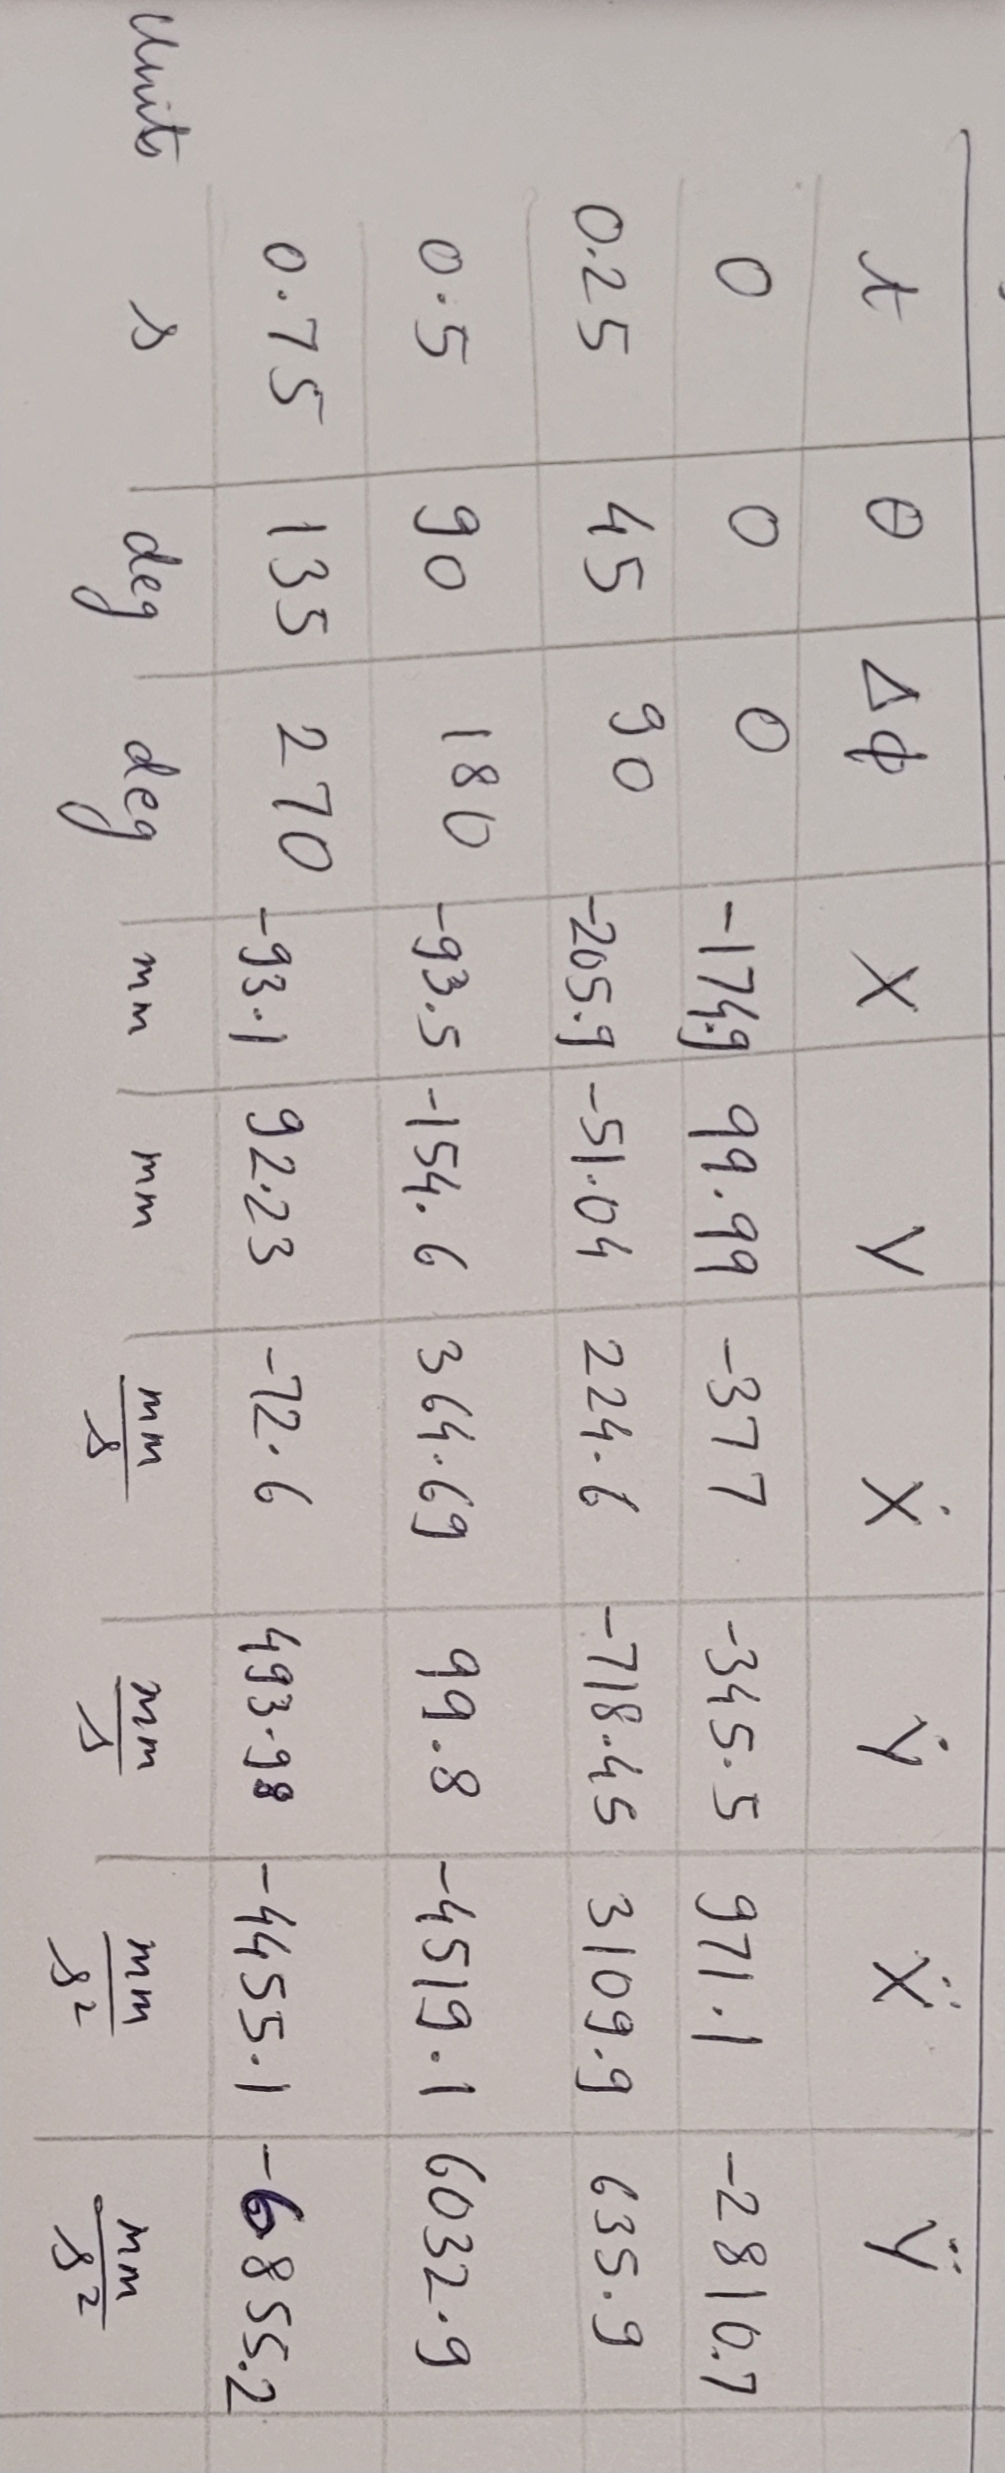
\includegraphics[width=0.9\columnwidth]{Images/theo_eval_result.jpg}
            \caption{Theoretical evaluation result}
            \label{fig:theo_eval_result}
        \end{figure}

        \begin{figure}[hbt!]
            \centering
            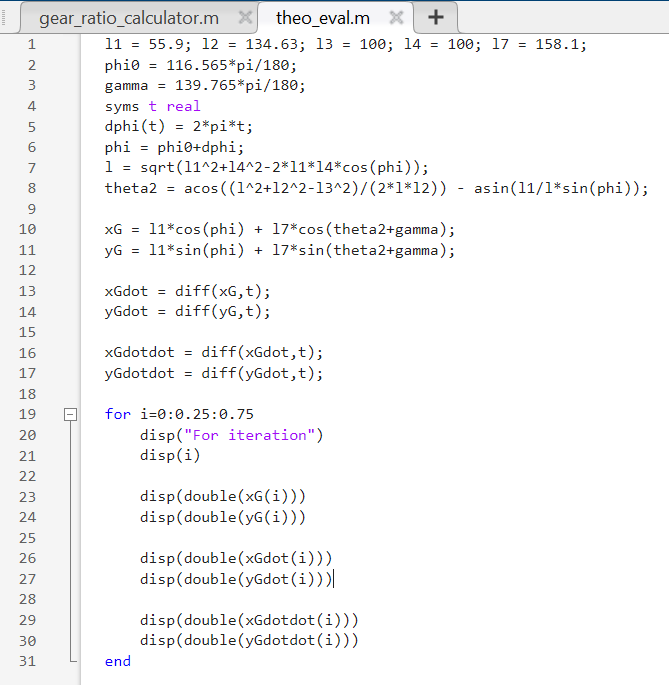
\includegraphics[width=0.9\columnwidth]{Images/matlab_script.png}
            \caption{MATLAB script used for calculating the analytical kinematics}
            \label{fig:matlab_script}
        \end{figure}

        These are displayed in fig~\ref{fig:theo_eval1}, fig~\ref{fig:theo_eval2}, fig~\ref{fig:theo_eval3} fig~\ref{fig:theo_eval_result} and MATLAB script is attached in fig~\ref{fig:matlab_script}.

    \subsection{Comparison of kinematic parameters}
        \subsubsection{Displacement}
            The four values of displacement evaluated in section 3.1 superimposed in the plot of section 2.1.1. Refer fig~\ref{fig:theo_eval1}, fig~\ref{fig:theo_eval2} and fig~\ref{fig:theo_eval3} for displacement calculation analytically. 

            \begin{figure}[hbt!]
                \centering
                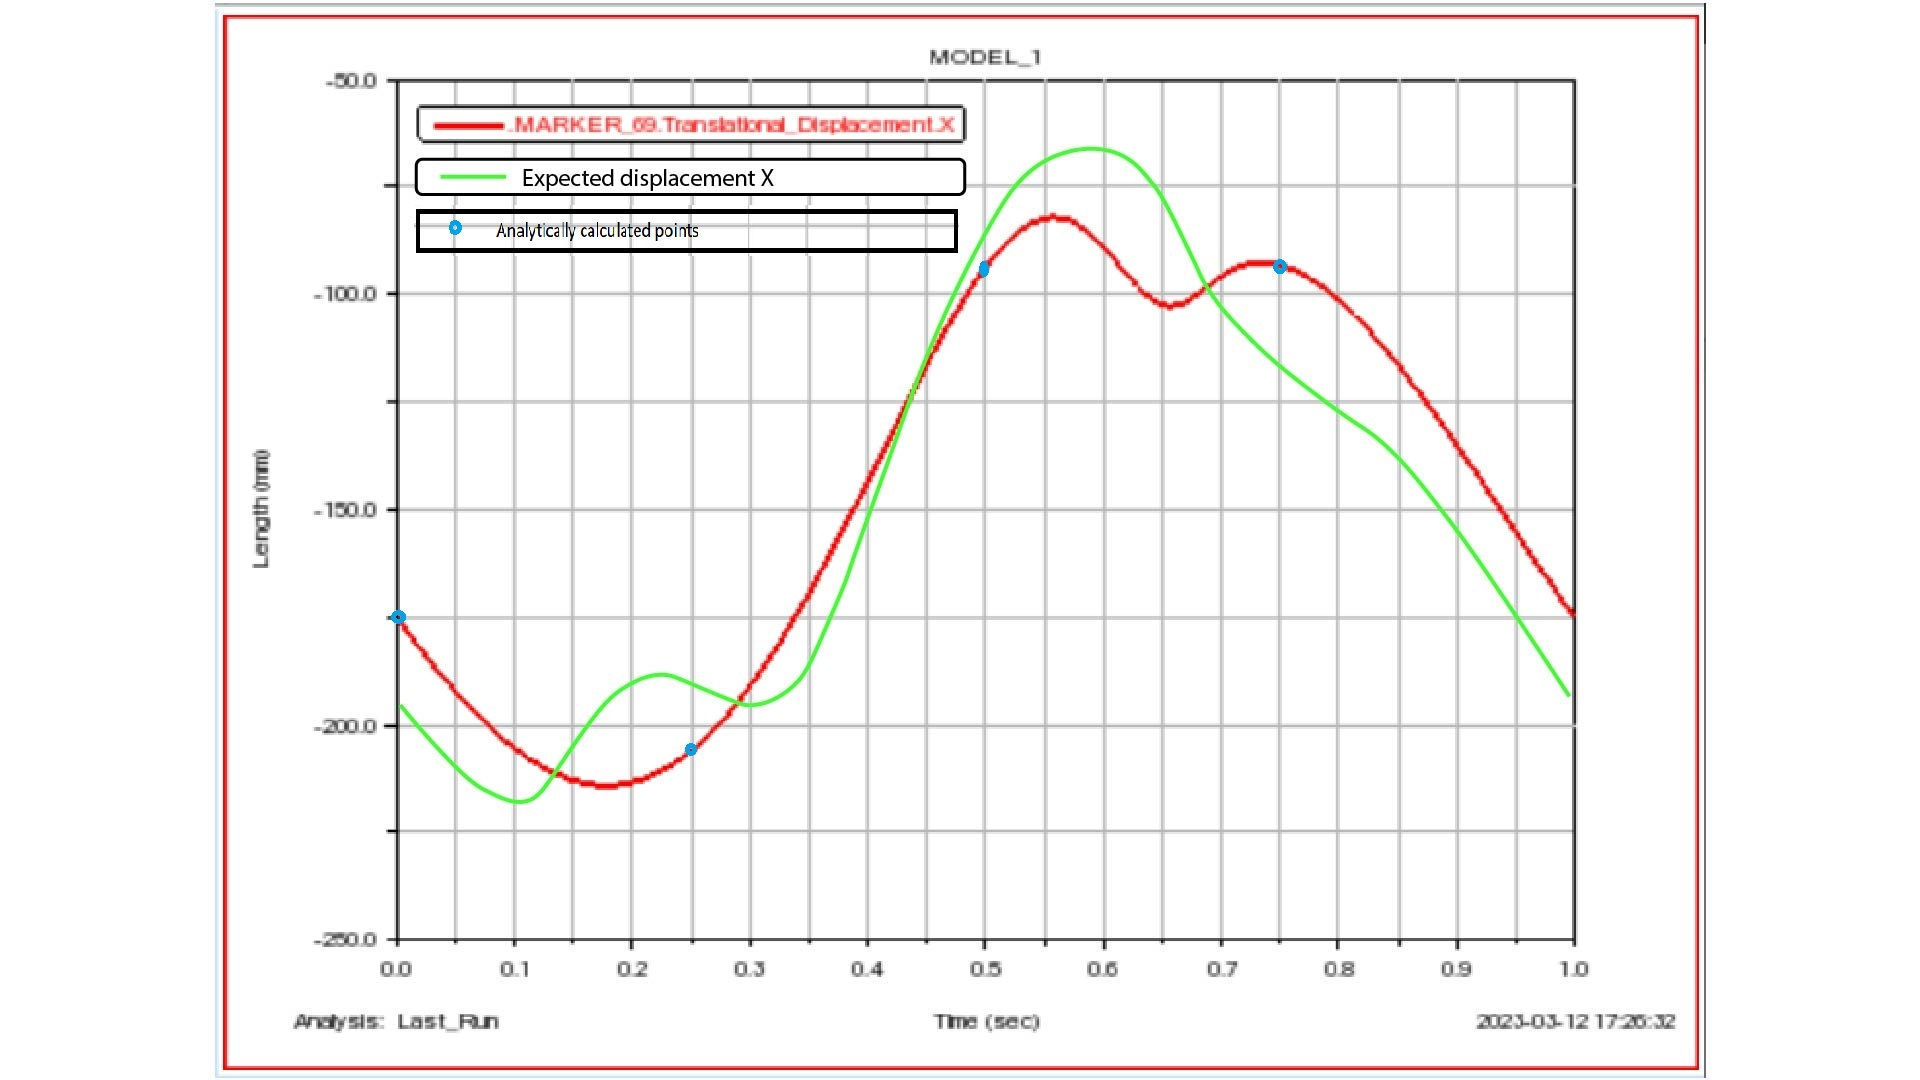
\includegraphics[width=0.9\columnwidth]{Images/anal_x_disp.jpg}
                \caption{Superimposed X displacement}
                \label{fig:anal_x_disp}
            \end{figure}

            \begin{figure}[hbt!]
                \centering
                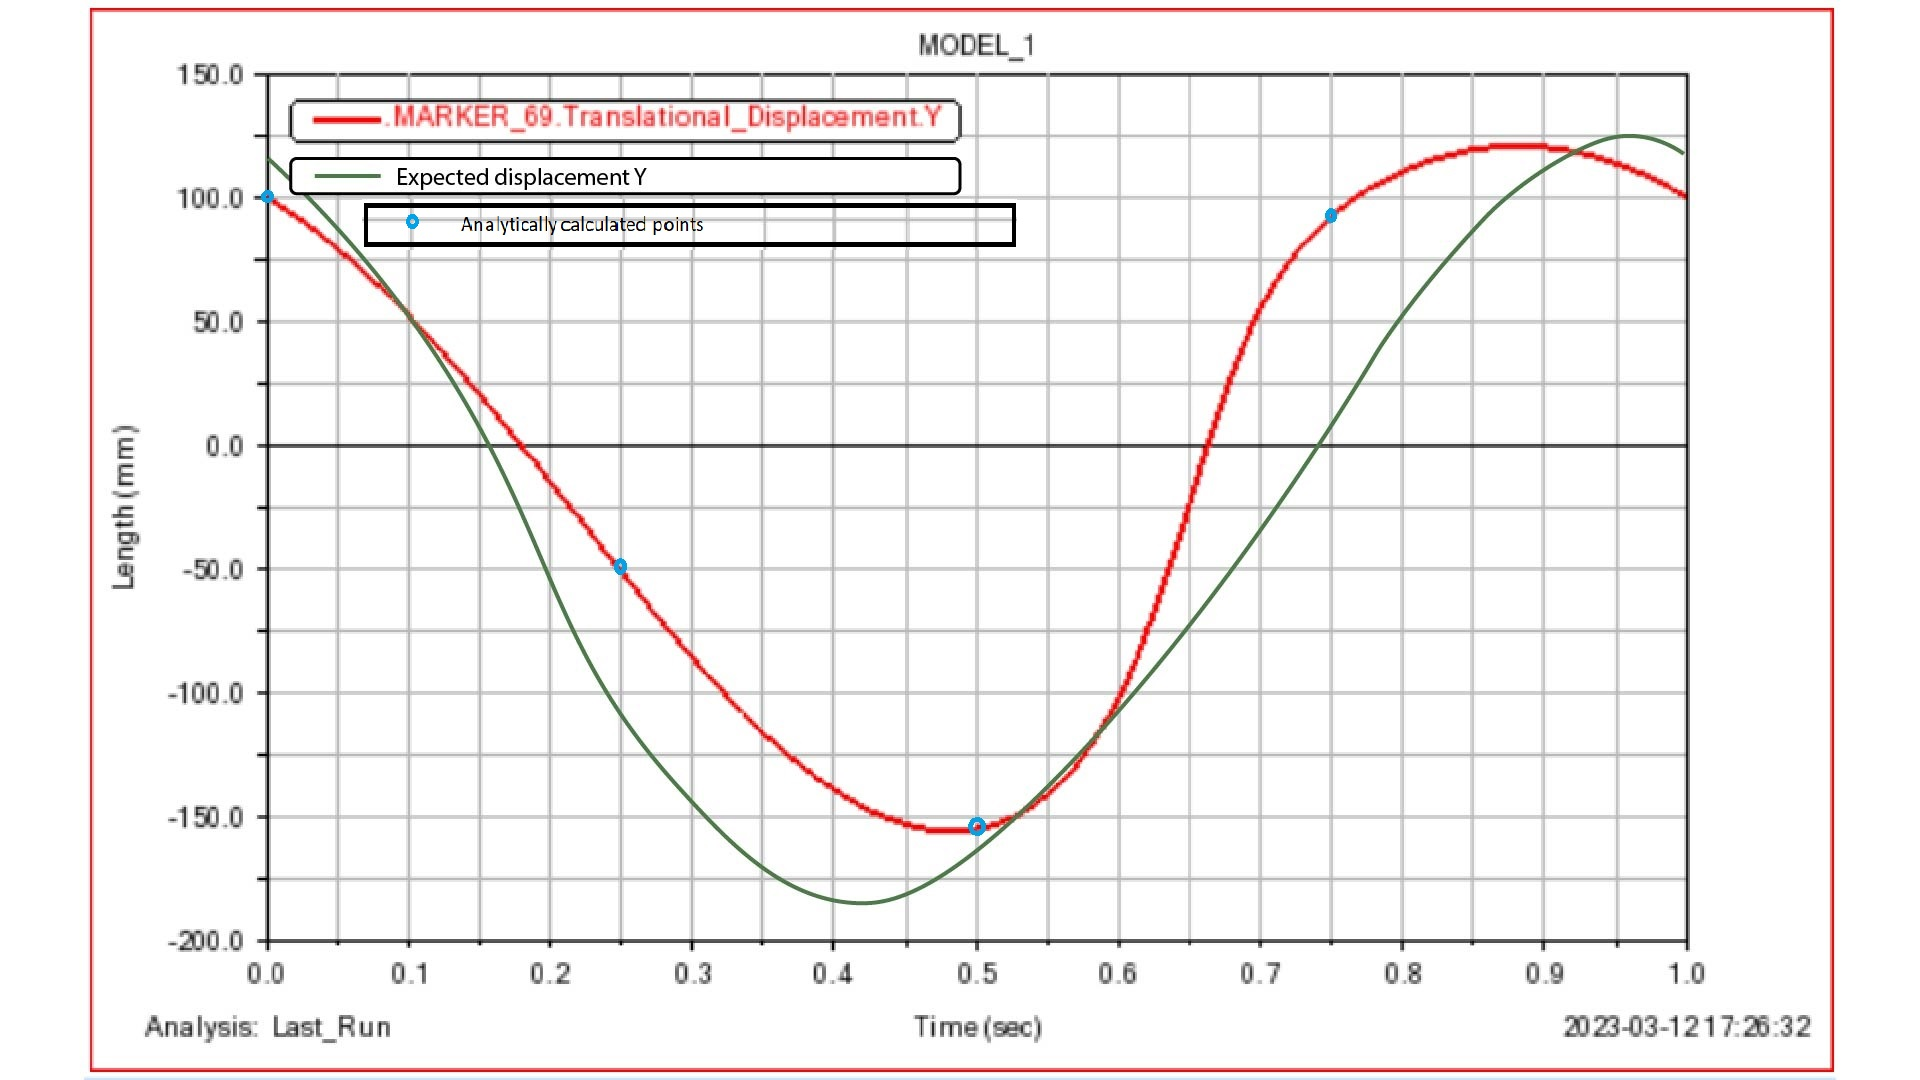
\includegraphics[width=0.9\columnwidth]{Images/anal_height_variation.jpg}
                \caption{Superimposed Y displacement}
                \label{fig:anal_y_disp}
            \end{figure}

            For superimposed graphs refer fig~\ref{fig:anal_x_disp} and fig~\ref{fig:anal_y_disp}.

        \subsubsection{Velocity}
            The four values of velocity evaluated in section 3.1 superimposed in the plot of section 2.1.2. Refer fig~\ref{fig:theo_eval_result} for analytical velocity result.

            \begin{figure}[hbt!]
                \centering
                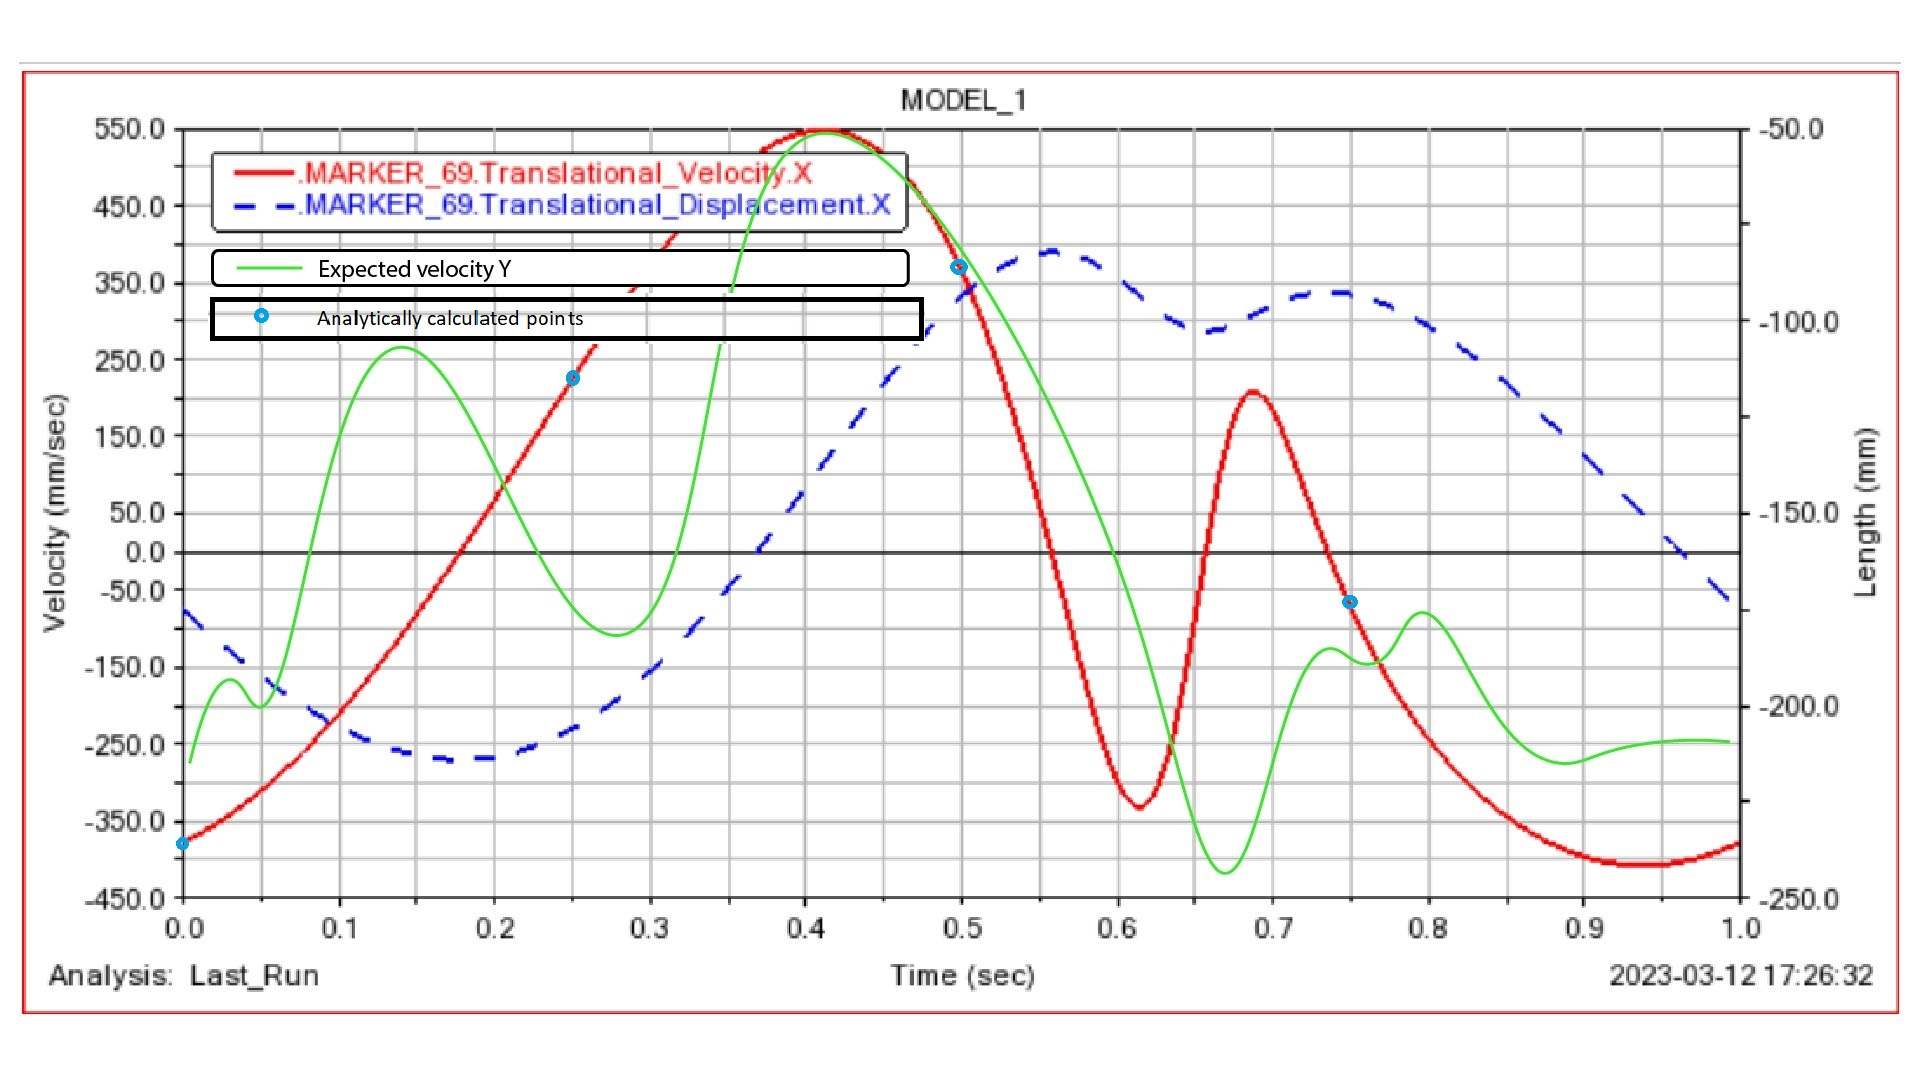
\includegraphics[width=0.9\columnwidth]{Images/anal_x_vel.jpg}
                \caption{Superimposed X vel}
                \label{fig:anal_x_vel}
            \end{figure}

            \begin{figure}[hbt!]
                \centering
                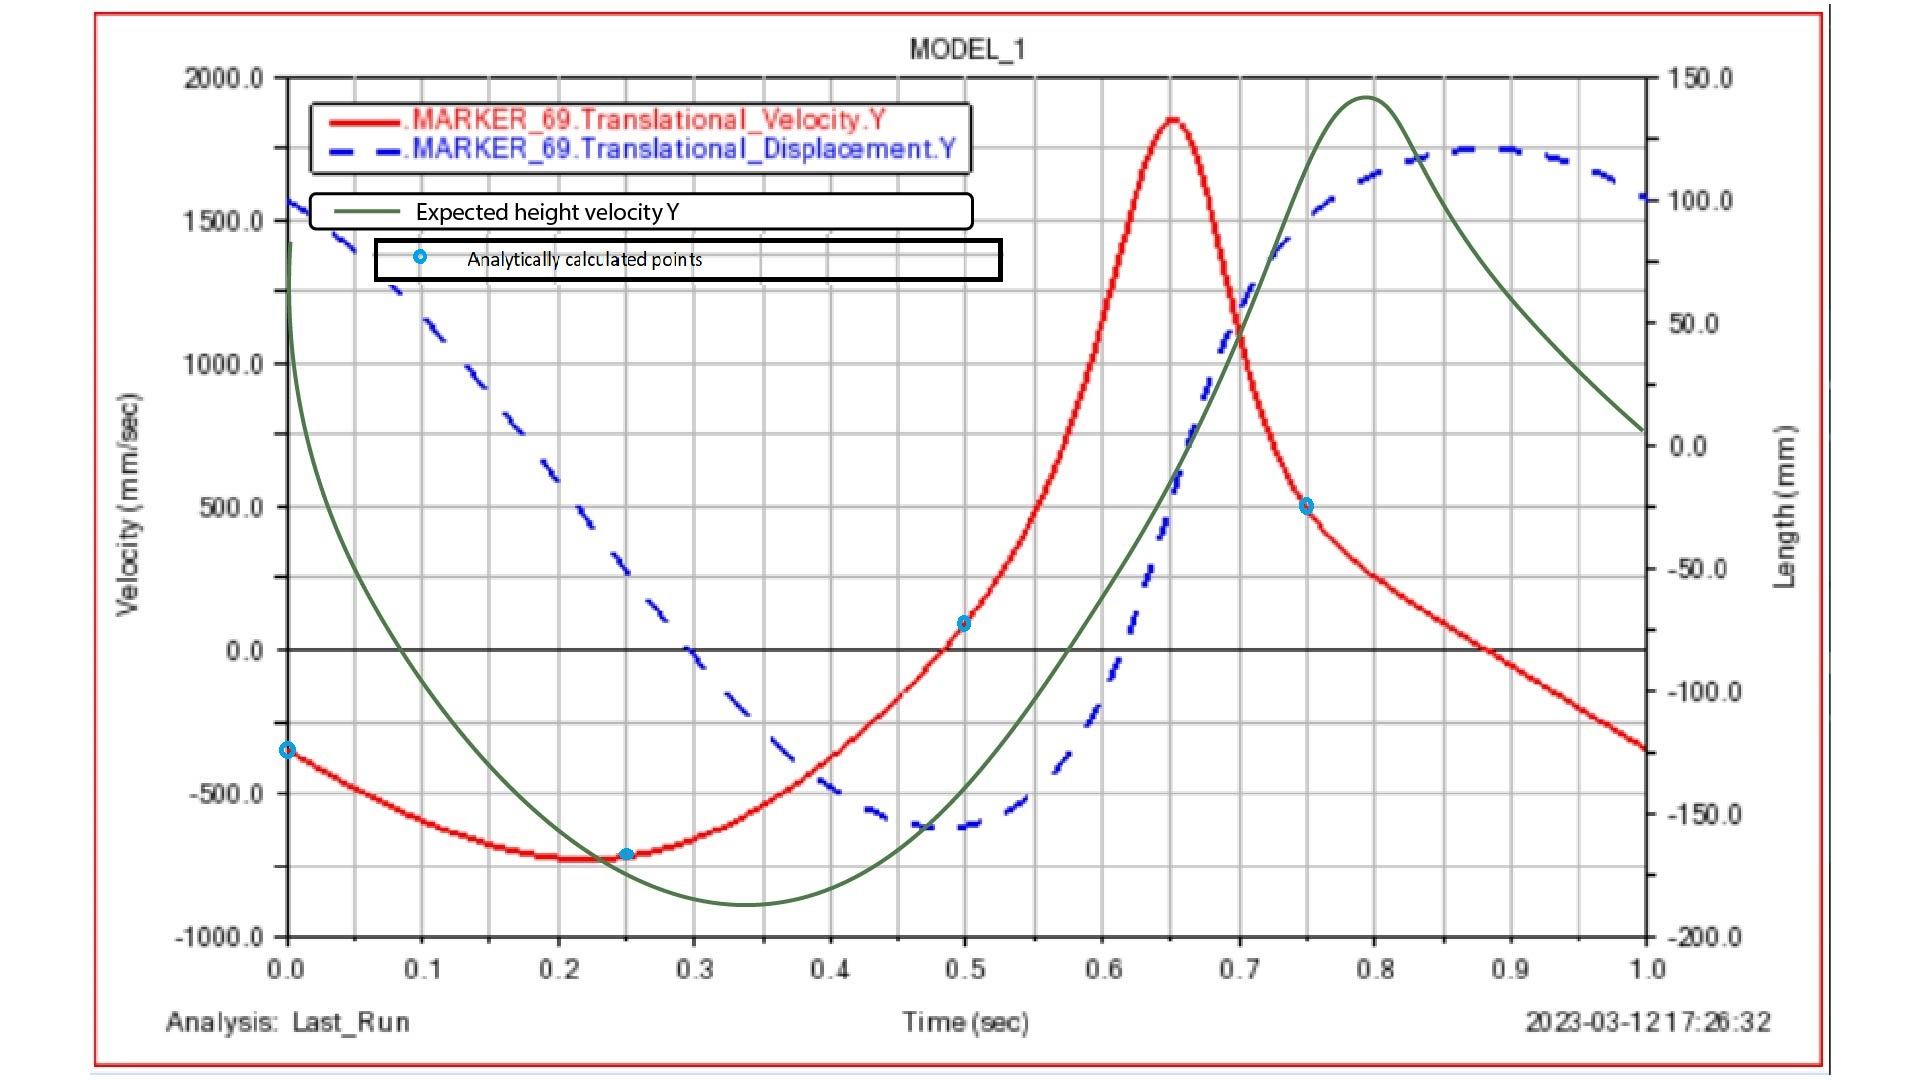
\includegraphics[width=0.9\columnwidth]{Images/anal_height_velocity.jpg}
                \caption{Superimposed Y vel}
                \label{fig:anal_y_vel}
            \end{figure}

            For superimposed graphs refer fig~\ref{fig:anal_x_vel} and fig~\ref{fig:anal_y_vel}.

        \subsubsection{Acceleration}
            The four values of velocity evaluated in section 3.1 superimposed in the plot of section 2.1.3. Refer fig~\ref{fig:theo_eval_result} for analytical acceleration result.

            \begin{figure}[hbt!]
                \centering
                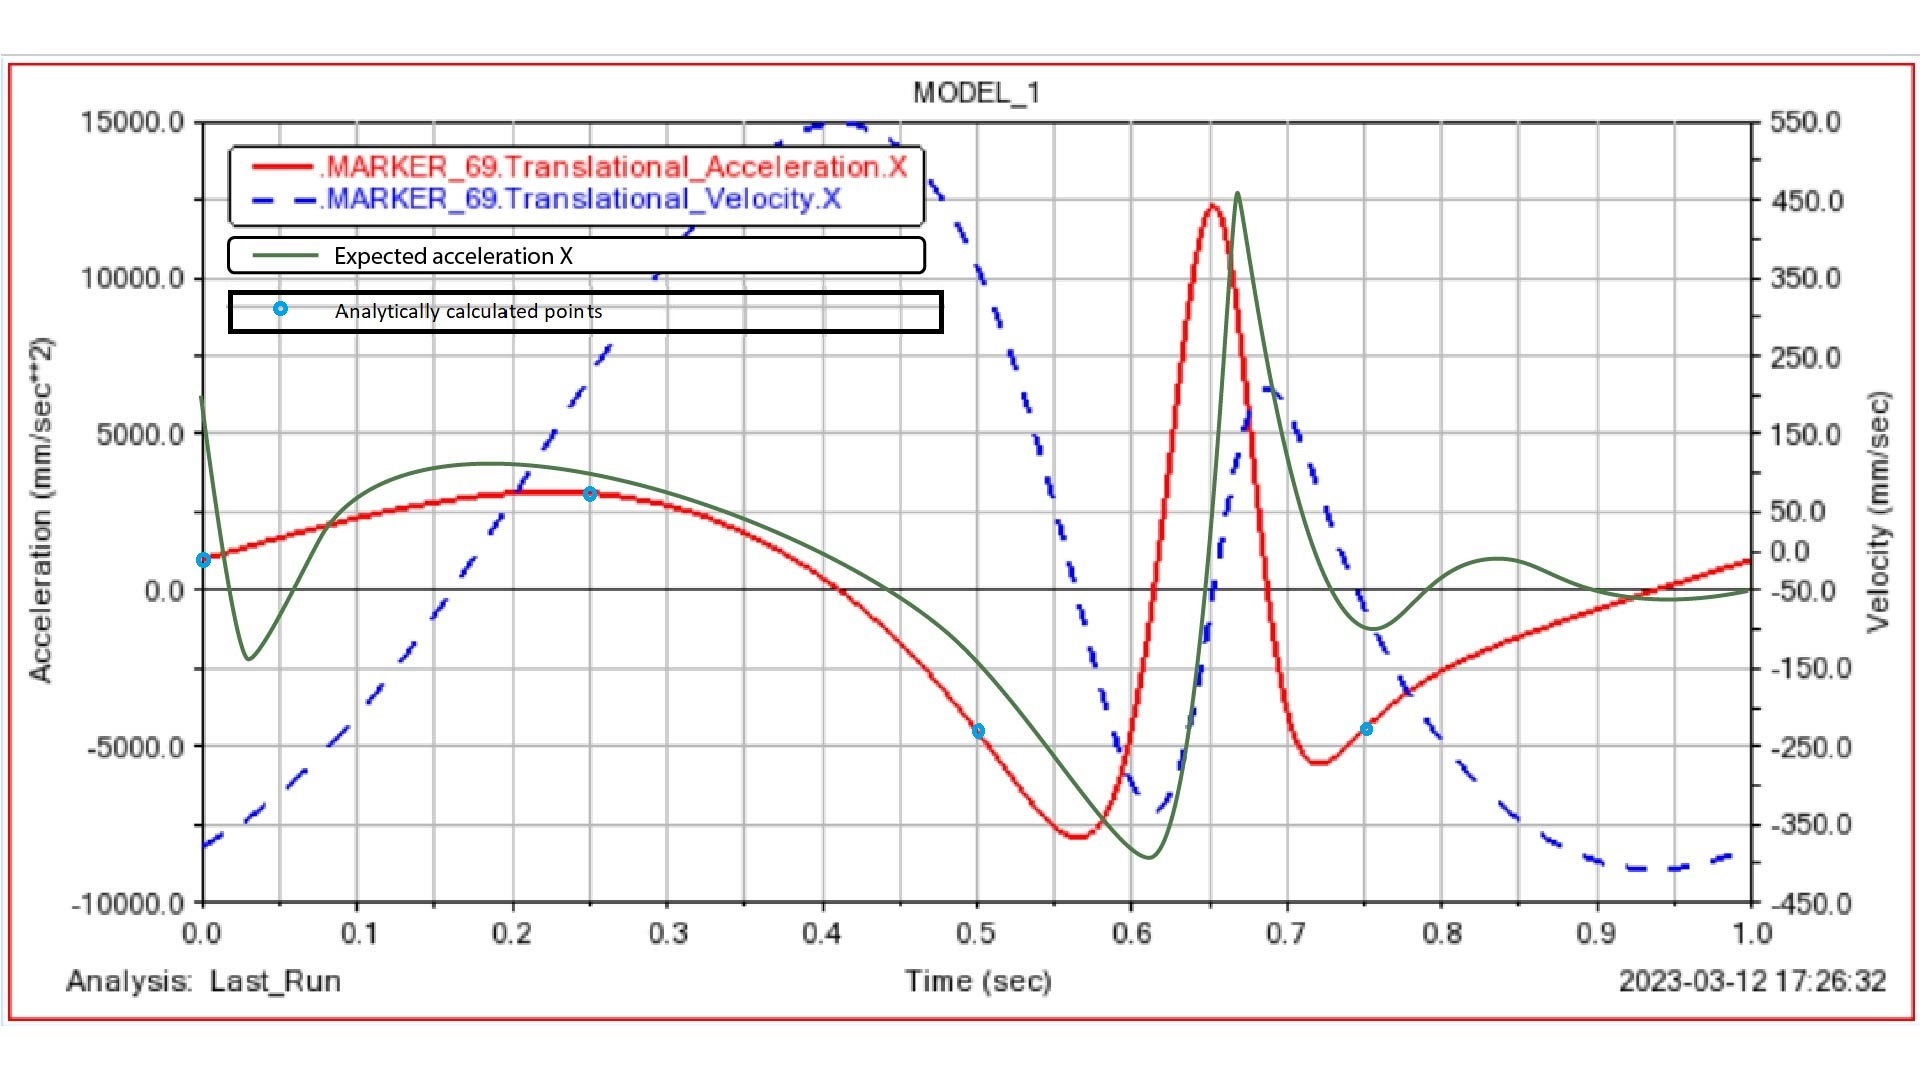
\includegraphics[width=0.9\columnwidth]{Images/anal_x_acc.jpg}
                \caption{Superimposed X acc}
                \label{fig:anal_x_acc}
            \end{figure}

            \begin{figure}[hbt!]
                \centering
                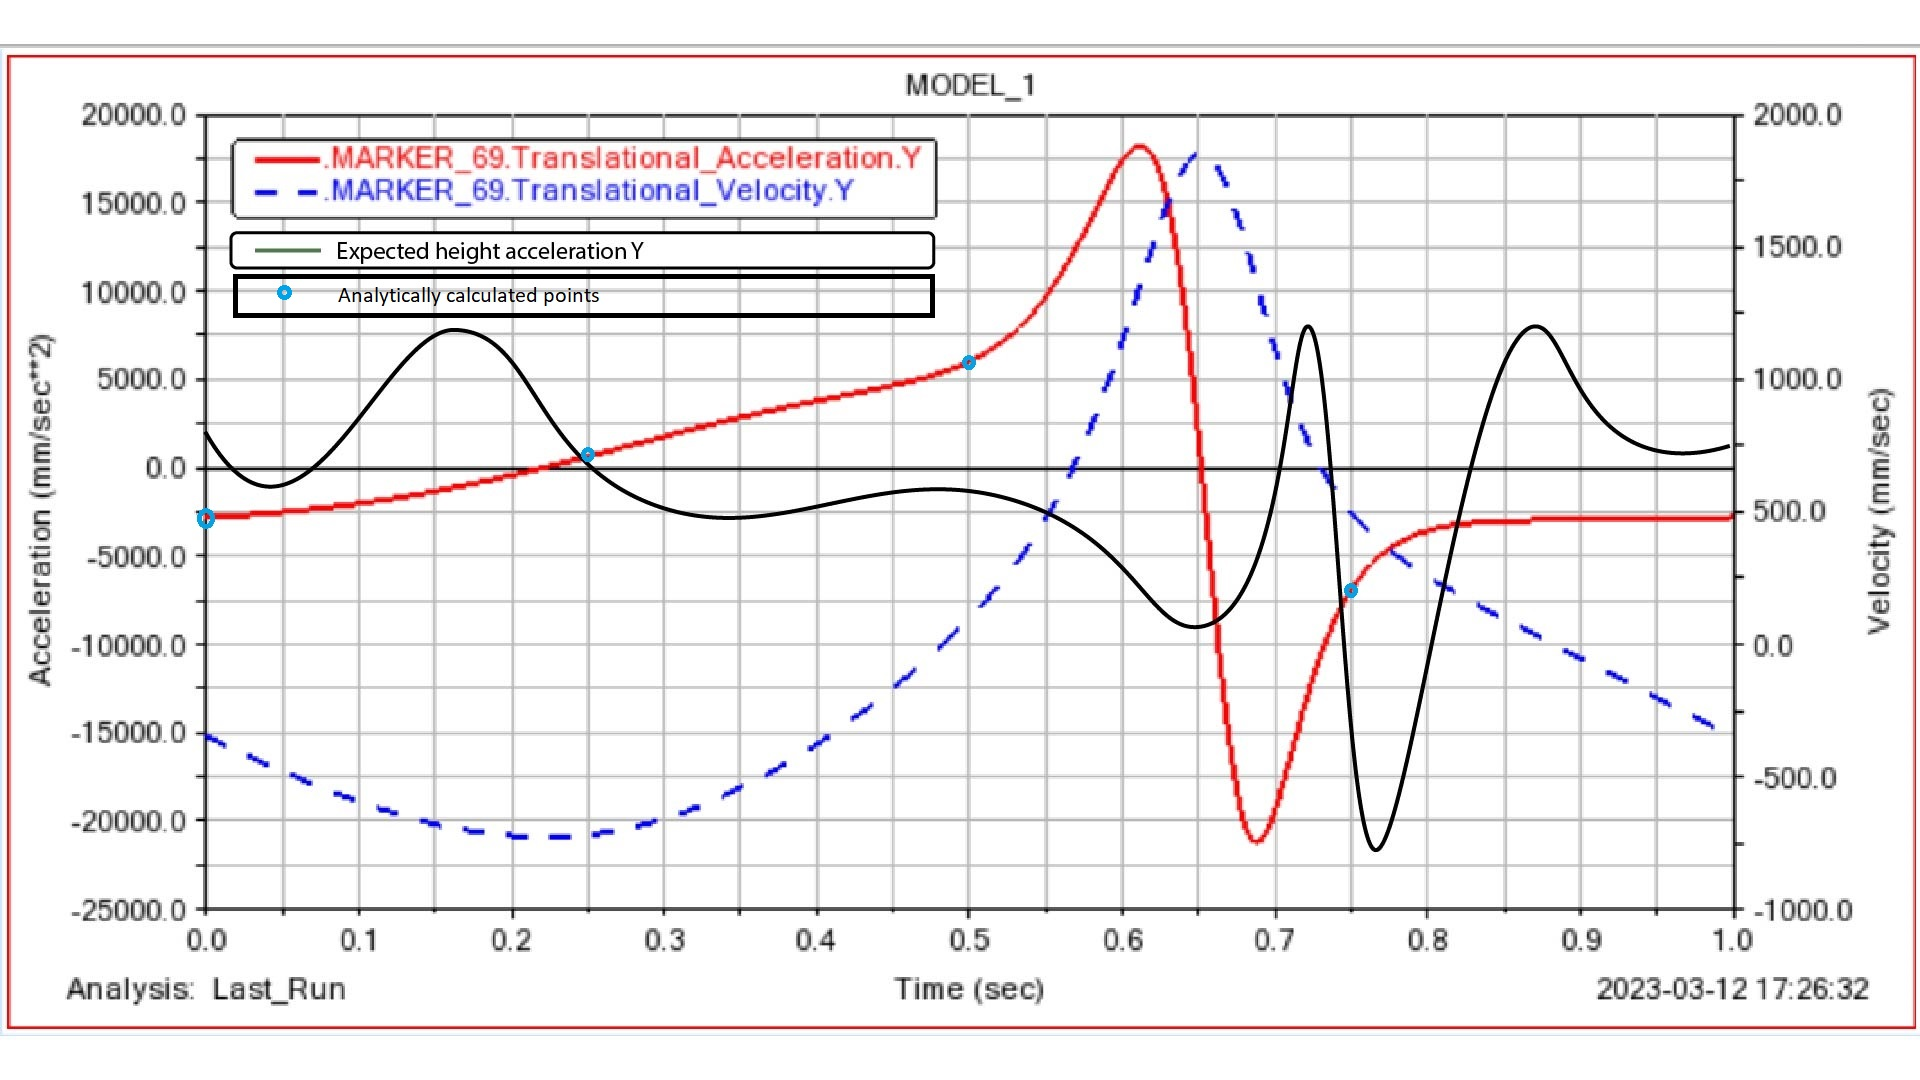
\includegraphics[width=0.9\columnwidth]{Images/anal_height_acceleration.jpg}
                \caption{Superimposed Y acc}
                \label{fig:anal_y_acc}
            \end{figure}

            For superimposed graphs refer fig~\ref{fig:anal_x_acc} and fig~\ref{fig:anal_y_acc}.

        \subsubsection{Comments}
            \begin{enumerate}
                \item There are minor differences in the calculations which can be due to two reasons.
                \item First being the rounding error while taking the values in MATLAB.
                \item Second being the simulation error where number of steps were a little low for generating these inaccuracies.
            \end{enumerate}